\subsubsection*{Zadanie~245.}
\begin{figure}[H]
    \centering
    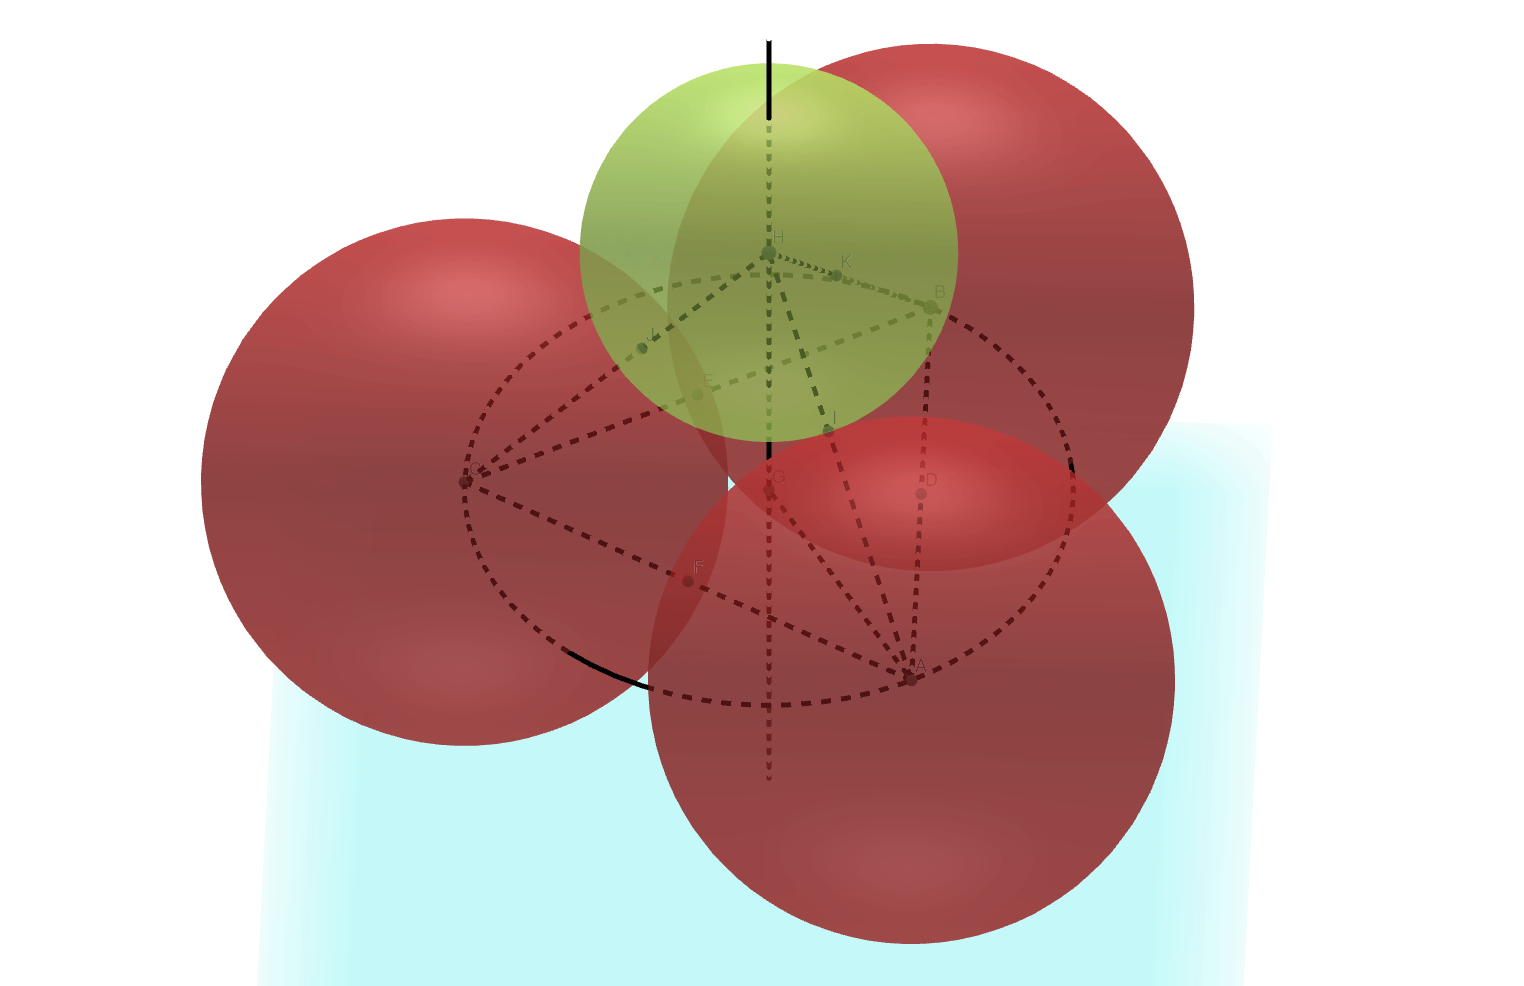
\includegraphics[width=\textwidth]{img/2021_03_01/245/space.png}
\end{figure}
Na początek obliczmy odległość środka czwartej kuli od stołu, później wystarczy dodać do tego \(r\). Zauważmy, że ponieważ trzy kule tworzące podstawę piramidy są identyczne, to ich środki, czyli punkty \(A\), \(B\), \(C\), wyznaczają wierzchołki trójkąta równobocznego o~boku \(2R\) w~płaszczyźnie równoległej do stołu i~odległej od niego o~\(R\). Ponieważ środek czwartej kuli jest równo odległy od środków pozostałych (dokładnie o~\(r + R\)) to musi leżeć na osi prostopadłej do płaszczyzny trójkąta \(\triangle{ABC}\) i~przechodzącej przez środek okręgu opisanego na nim. Jeśli oznaczymy środek czwartej kuli przez \(H\), a~środek okręgu opisanego na \(\triangle{ABC}\) przez \(G\), to \(\triangle{AGH}\) jest prostokątny. Z~własności trójkąta równobocznego wiemy, że
\begin{equation*}
    AG = \frac{2\sqrt{3}R}{3}
\end{equation*}
Możemy teraz wyliczyć z~twierdzenia Pitagorasa:
\begin{equation*}
    GH
    = \sqrt{AH^2 - AG^2}
    = \sqrt{\pars{R + r}^2 - \pars{\frac{2\sqrt{3}R}{3}}^2}
    = \sqrt{R^2 + 2Rr + r^2 - \frac{4R^2}{3}}
    = \sqrt{2Rr + r^2 - \frac{R^2}{3}}
\end{equation*}
Do tak wyliczonej odległości wystarczy dodać odległość punktu \(G\) od stołu oraz wspomnianą już długość promienia czwartej kuli. Zatem największa odległość punktu czwartej kuli od stołu wynosi
\begin{equation*}
    d = \sqrt{2Rr + r^2 - \frac{R^2}{3}} + R + r
\end{equation*}
Aby ustawienie piramidy było możliwe, sfera o~promieniu \(r\) musi ,,zatykać'' dziurę w~środku podstawy piramidy, czyli:
\begin{gather*}
    R + r \geq AG\\
    R + r \geq \frac{2\sqrt{3}R}{3}\\
    r \geq \frac{R\pars{2\sqrt{3} - 1}}{3}
\end{gather*}
\subsubsection*{Zadanie~246.}
Rozważmy przekrój osiowy tej konfiguracji:
\begin{mathfigure*}
    \coordinate (A) at (-3, 0);
    \coordinate (B) at (3, 0);
    \coordinate (C) at (0, 6);
    \coordinate (I) at (0, 1.85);
    \coordinate (E) at (1.66, 2.68);
    \coordinate (D) at (0, 0);
    \drawangle[Orange]{D--C--B};
    \drawangle*[RoyalBlue]{E--I--C}[\(\alpha\)];
    \drawangle*[RoyalBlue]{C--B--D}[\(\alpha\)];
    \draw (I) circle[radius=1.85];
    \draw (C) -- node[left]{\(h\)} (D);
    \draw (I) -- node[above, sloped]{\(r\)} (E);
    \path (I) -- node[left]{\(r\)} (D);
    \draw (A) -- node[pos=0.75, below]{\(R\)} (B) -- (C) -- node[above left]{\(\ell\)} cycle;
    \drawrightangle{B--D--C};
    \drawrightangle{C--E--I};
    \fillpoint*{A}[\(A\)][below left];
    \fillpoint*{B}[\(B\)][below right];
    \fillpoint*{C}[\(C\)][above];
    \fillpoint*{I}[\(I\)][below left];
    \fillpoint*{E}[\(E\)][above right];
    \fillpoint*{D}[\(D\)][below];
\end{mathfigure*}
\begin{gather*}
    \triangle{EIC} \sim \triangle{DBC}\\
    \frac{r}{h - r} = \frac{R}{\ell}\\
    R\pars{h - r} = r\ell\\
    Rh - Rr = r\ell\\
    rR + r\ell = Rh\\
    r\pars{R + \ell} = Rh\\
    r = \frac{Rh}{R + \ell}\\
    S_\p{podstawy} = \pi R^2\\
    S_\p{kuli} = 4\pi r^2 = 4\pi\frac{R^2h^2}{\pars{R + \ell}^2}\\
    S_\p{boczna} = \pi R\ell\\
    2 \cdot S_\p{kuli} = S_\p{podstawy} + S_\p{boczna}\\
    8\pi\frac{R^2h^2}{\pars{R + \ell}^2} = \pi R\pars{R + \ell}\\
    \frac{8Rh^2}{\pars{R + \ell}^2} = R + \ell\\
    8Rh^2 = \pars{R + \ell}^3\\
    8R\pars{\ell^2 - R^2} = R^3 + 3R^2\ell + 3R\ell^2 + \ell^3\\
    8R\ell^2 - 8R^3 = R^3 + 3R^2\ell + 3R\ell^2 + \ell^3\\
    9R^3 + 3R^2\ell - 5R\ell^2 + \ell^3 = 0\\
    \pars{R + \ell}\pars{9R^2 - 6R\ell + \ell^2} = 0\\
    \pars{R + \ell}\pars{3R - \ell}^2 = 0\\
    R = -\ell < 0 \wrong \wlor R = \frac{\ell}{3} \ok\\
    \cos\alpha = \frac{R}{\ell} = \frac{\frac{\ell}{3}}{\ell} = \frac{1}{3}
\end{gather*}
\subsubsection*{Zadanie~247.}
\begin{mathfigure*}
    \coordinate (A) at (-2, -0.4);
    \coordinate (B) at (1, -0.4);
    \coordinate (C) at (2, 0.4);
    \coordinate (D) at (-1, 0.4);
    \coordinate (Aprime) at (-2, 3.6);
    \coordinate (Bprime) at (1, 3.6);
    \coordinate (Cprime) at (2, 4.4);
    \coordinate (Dprime) at (-1, 4.4);
    \coordinate (E) at ($(A)!0.5!(C)$);
    \draw (A) -- node[below]{\(a\)} (B) -- node[below, sloped]{\(a\)} (C);
    \draw[dashed] (C) -- (D) -- (A);
    \draw[dashed] (D) -- (Dprime);
    \drawangle*[Orange]{A--Dprime--C}[\(\alpha\)];
    \draw[Orange] (A) -- node[above, sloped]{\(d\)} (Dprime) -- node[above, sloped]{\(d\)} (C) -- cycle;
    \drawrightangle[angle radius=0.3cm]{C--E--Dprime};
    \draw[dotted] (Dprime) -- node[right]{\(x\)} (E);
    \draw (A) -- (Aprime);
    \draw (B) -- (Bprime);
    \draw (C) -- node[right]{\(h\)} (Cprime);
    \draw (Aprime) -- (Bprime) -- (Cprime) -- (Dprime) -- cycle;
    \fillpoint*{A}[\(A\)][below left];
    \fillpoint*{B}[\(B\)][below right];
    \fillpoint*{C}[\(C\)][above right];
    \fillpoint*{D}[\(D\)][above left];
    \fillpoint*{Aprime}[\(A'\)][above left];
    \fillpoint*{Bprime}[\(B'\)][below right];
    \fillpoint*{Cprime}[\(C'\)][above right];
    \fillpoint*{Dprime}[\(D'\)][above];
    \fillpoint*{E}[\(E\)][below right];
\end{mathfigure*}
Na rysunku \(E\) jest środkiem podstawy \(ABCD\). Ponieważ ściany boczne są przystające, a~odcinki \(AD'\) i~\(CD'\) są ich przekątnymi, to \(\triangle{ACD'}\) jest równoramienny.
\begin{gather*}
    S
    = 2 \cdot \frac{1}{2} \cdot ah + \frac{1}{2}a^2 + \area{ACD'}
    = ah + \frac{a^2}{2} + \area{ACD'}\\
    S_\p{graniastosłupa}
    = 4ah + 2a^2
    = 4\pars{ah + \frac{a^2}{2}}
    = 4\pars{S - \area{ACD'}}
\end{gather*}
Odcinek \(EC\) ma długość \(\frac{a\sqrt{2}}{2}\), jako połowa przekątnej podstawy. Możemy zapisać zależności trygonometryczne dla \(\triangle{CED'}\):
\begin{gather*}
    \frac{D'E}{EC} = \cot\frac{\alpha}{2}\\
    \frac{x}{\frac{a\sqrt{2}}{2}} = \cot\frac{\alpha}{2}\\
    x = \frac{a\sqrt{2}}{2}\cot\frac{\alpha}{2}\\
    \area{ACD'} = \frac{1}{2} \cdot a\sqrt{2} \cdot x
    = \frac{a^2\cot\frac{\alpha}{2}}{2}
\end{gather*}
Możemy także zapisać:
\begin{gather*}
    \frac{\frac{a\sqrt{2}}{2}}{d} = \sin\frac{\alpha}{2}\\
    d = \frac{a\sqrt{2}}{2\sin\frac{\alpha}{2}}\\
    h
    = \sqrt{d^2 - a^2}
    = \sqrt{\frac{a^2}{2\sin^2\frac{\alpha}{2}} - a^2}
    = a\sqrt{\frac{1}{2\sin^2\frac{\alpha}{2}} - 1}
\end{gather*}
Po podstawieniu wyliczonych wartości do wzoru na \(S\) otrzymujemy:
\begin{gather*}
    S
    = ah + \frac{a^2}{2} + \area{ACD'}
    = a^2\sqrt{\frac{1}{2\sin^2\frac{\alpha}{2}} - 1} + \frac{a^2}{2} + \frac{a^2\cot\frac{\alpha}{2}}{2}
    = a^2\pars{\sqrt{\frac{1}{2\sin^2\frac{\alpha}{2}} - 1} + \frac{1 + \cot\frac{\alpha}{2}}{2}}\\
    a^2 = \frac{S}{\sqrt{\frac{1}{2\sin^2\frac{\alpha}{2}} - 1} + \frac{1 + \cot\frac{\alpha}{2}}{2}}
\end{gather*}
Możemy teraz wyznaczyć pole powierzchni całkowitej graniastosłupa:
\begin{equation*}
    \begin{split}
        S_\p{graniastosłupa}
        &= 4\pars{S - \area{ACD'}}
        = 4\pars{S - \frac{a^2\cot\frac{\alpha}{2}}{2}}
        = 4\pars{S - \frac{S\cot\frac{\alpha}{2}}{2\sqrt{\frac{1}{2\sin^2\frac{\alpha}{2}} - 1} + \cot\frac{\alpha}{2} + 1}}\\
        &= 4S\pars{1 - \frac{\cot\frac{\alpha}{2}}{2\sqrt{\frac{1}{2\sin^2\frac{\alpha}{2}} - 1} + \cot\frac{\alpha}{2} + 1}}
    \end{split}
\end{equation*}
\subsubsection*{Zadanie~248.}
W~ostrosłupie prawidłowym środek kuli wpisanej leży na wysokości. Przez \(E\) oznaczmy środek jednej z~krawędzi podstawy.
\begin{mathfigure*}
    \coordinate (A) at (-4, 0);
    \coordinate (B) at (2, 0);
    \coordinate (C) at (0, 1);
    \coordinate (S) at (-1, 6);
    \coordinate (I) at (-1, 1.76);
    \coordinate (E) at ($(B)!0.5!(C)$);
    \coordinate (H) at (-1, 0.32);
    \coordinate (T) at (0.375, 2.2);
    \coordinate (P) at ($(A)!1.22!(E)$);
    \draw[ForestGreen] (H) ellipse (3.35 and 0.73);
    \drawangle*[ForestGreen]{A--S--P}[\(\alpha\)];
    \draw (A) -- node[below]{\(a\)} (B);
    \draw[dashed] (B) -- (C) -- (A);
    \draw[dotted] (E) -- (P);
    \draw[ForestGreen] (P) -- (S);
    \draw[dashed] (S) -- (C);
    \draw[Orange] (I) circle[radius=1.44];
    \draw[dotted] (S) -- node[left]{\(h\)} (H);
    \draw[Orange, densely dotted] (I) ellipse (1.44 and 0.2);
    \drawrightangle[angle radius=0.3cm]{E--H--S};
    \drawrightangle[angle radius=0.4cm]{S--E--C};
    \draw (S) -- (A);
    \draw (S) -- (B);
    \draw[RoyalBlue, dashed] (A) -- (E) -- (S) -- cycle;
    \fillpoint*[1][RoyalBlue][RoyalBlue]{E}[\(E\)][right];
    \fillpoint*[1][RoyalBlue][RoyalBlue]{A}[\(A\)][below left];
    \fillpoint*[1][RoyalBlue][RoyalBlue]{S}[\(S\)][above];
    \fillpoint*[1][RoyalBlue][RoyalBlue]{H}[\(H\)][above left];
    \fillpoint*[1][RoyalBlue][RoyalBlue]{T}[\(T\)][above right];
    \fillpoint*[1][Orange][Orange]{I}[\(I\)][above left];
    \fillpoint*[1][ForestGreen][ForestGreen]{P}[\(P\)][above right];
\end{mathfigure*}
\noindent
Podstawą stożka jest koło opisane na podstawie ostrosłupa. Z~własności trójkąta równobocznego wiemy, że jego promień wynosi \(\frac{a\sqrt{3}}{3}\), jeśli przez \(a\) oznaczymy długość krawędzi podstawy. Rozważmy przekrój osiowy stożka:
\begin{mathfigure*}
    \coordinate (A) at (-3, 0);
    \coordinate (P) at (3, 0);
    \coordinate (S) at (0, 6);
    \coordinate (H) at (0, 0);
    \drawrightangle[angle radius=0.4cm]{P--H--S};
    \drawangle*[ForestGreen]{A--S--P}[\(\alpha\)];
    \drawangle*[RoyalBlue]{P--A--S}[\(\beta\)];
    \draw[ForestGreen] (A) -- node[pos=0.75, below]{\(\frac{a\sqrt{3}}{3}\)} (P) -- node[sloped]{\(|\)} (S) -- node[sloped]{\(|\)} cycle;
    \draw[dotted] (S) -- node[left]{\(h\)} (H);
    \fillpoint*[1][RoyalBlue][RoyalBlue]{A}[\(A\)][below left];
    \fillpoint*[1][ForestGreen][ForestGreen]{P}[\(P\)][below right];
    \fillpoint*[1][ForestGreen][ForestGreen]{S}[\(S\)][above];
    \fillpoint*{H}[\(H\)][below];
\end{mathfigure*}
\noindent
\begin{gather*}
    \frac{h}{\frac{a\sqrt{3}}{3}} = \cot\frac{\alpha}{2}\\
    h = \frac{a\sqrt{3}\cot\frac{\alpha}{2}}{3}
\end{gather*}
Znając wysokość, możemy już obliczyć objętości ostrosłupa i~stożka:
\begin{gather*}
    V_\p{ostrosłupa}
    = \frac{1}{3} \cdot \frac{a^2\sqrt{3}}{4} \cdot \frac{a\sqrt{3}\cot\frac{\alpha}{2}}{3}
    = \frac{a^3\cot\frac{\alpha}{2}}{12}\\
    V_\p{stożka}
    = \frac{1}{3} \cdot \pi \pars{\frac{a\sqrt{3}}{3}}^2 \cdot h
    = \frac{1}{3} \cdot \pi \cdot \frac{a^2}{3} \cdot \frac{a\sqrt{3}\cot\frac{\alpha}{2}}{3}
    = \frac{a^3\pi\sqrt{3}\cot\frac{\alpha}{2}}{27}
\end{gather*}
Musimy jeszcze znaleźć pole powierzchni całkowitej ostrosłupa. W~tym celu wyznaczmy wysokość ściany bocznej:
\begin{equation*}
    SE
    = \sqrt{HE^2 + HS^2}
    = \sqrt{\pars{\frac{a\sqrt{3}}{6}}^2 + \pars{\frac{a\sqrt{3}\cot\frac{\alpha}{2}}{3}}^2}
    = \sqrt{\frac{a^2}{12} + \frac{a^2\cot^2\frac{\alpha}{2}}{3}}
    = \frac{a}{2}\sqrt{\frac{1 + 4\cot^2\frac{\alpha}{2}}{3}}
\end{equation*}
Teraz możemy wyznaczyć pole powierzchni całkowitej ostrosłupa:
\begin{equation*}
    S_\p{ostrosłupa}
    = \frac{a^2\sqrt{3}}{4} + 3 \cdot \frac{1}{2} \cdot a \cdot SE
    = \frac{a^2\sqrt{3}}{4} + \frac{3}{4}a^2\sqrt{\frac{1 + 4\cot^2\frac{\alpha}{2}}{3}}
    = \frac{a^2\sqrt{3}}{4}\pars{1 + \sqrt{1 + 4\cot^2\frac{\alpha}{2}}}
\end{equation*}
Wyznaczamy szukane stosunki:
\begin{gather*}
    \begin{split}
        \frac{V_\p{kuli}}{V_\p{ostrosłupa}}
        &= \frac{\frac{4}{3}\pi R^3}{V_\p{ostrosłupa}}
        = \frac{\frac{4}{3}\pi\pars{\frac{3 \cdot V_\p{ostrosłupa}}{S_\p{ostrosłupa}}}^3}{V_\p{ostrosłupa}}
        = \frac{36\pi \cdot V_\p{ostrosłupa}^2}{S_\p{ostrosłupa}^3}
        = \frac{36\pi \cdot \frac{a^6\cot^2\frac{\alpha}{2}}{144}}{\frac{3\sqrt{3}a^6}{64}\pars{1 + \sqrt{1 + 4\cot^2\frac{\alpha}{2}}}^3}\\
        &= \frac{\frac{\pi\cot^2\frac{\alpha}{2}}{4}}{\frac{3\sqrt{3}}{64}\pars{1 + \sqrt{1 + 4\cot^2\frac{\alpha}{2}}}^3}
        = \frac{16\pi\cot^2\frac{\alpha}{2}}{3\sqrt{3}\pars{1 + \sqrt{1 + 4\cot^2\frac{\alpha}{2}}}^3}
    \end{split}\\
    \begin{split}
        \frac{V_\p{kuli}}{V_\p{stożka}}
        &= \frac{V_\p{kuli}}{V_\p{ostrosłupa}} \cdot \frac{V_\p{ostrosłupa}}{V_\p{stożka}}
        = \frac{16\pi\cot^2\frac{\alpha}{2}}{3\sqrt{3}\pars{1 + \sqrt{1 + 4\cot^2\frac{\alpha}{2}}}^3} \cdot \frac{\frac{a^3\cot\frac{\alpha}{2}}{12}}{\frac{a^3\pi\sqrt{3}\cot\frac{\alpha}{2}}{27}}
        = \frac{16\pi\cot^2\frac{\alpha}{2}}{3\sqrt{3}\pars{1 + \sqrt{1 + 4\cot^2\frac{\alpha}{2}}}^3} \cdot \frac{\frac{1}{12}}{\frac{\pi\sqrt{3}}{27}}\\
        &= \frac{4\cot^2\frac{\alpha}{2}}{\pars{1 + \sqrt{1 + 4\cot^2\frac{\alpha}{2}}}^3} \cdot \frac{}{}
    \end{split}
\end{gather*}
\subsubsection*{Zadanie~249.}
W~ostrosłupie prawidłowym środek kuli wpisanej leży na wysokości. Rozważmy następujący przekrój tego czworościanu (punkt \(E\) jest środkiem krawędzi podstawy, na której leży):
\begin{mathfigure*}
    \coordinate (A) at (-4, 0);
    \coordinate (B) at (2, 0);
    \coordinate (C) at (0, 1);
    \coordinate (S) at (-1, 6);
    \coordinate (I) at (-1, 1.76);
    \coordinate (E) at ($(B)!0.5!(C)$);
    \coordinate (H) at (-1, 0.32);
    \coordinate (T) at (0.375, 2.2);
    \drawangle*[RoyalBlue]{S--E--A}[\footnotesize\(2\alpha\)];
    \draw (A) -- node[below]{\(a\)} (B);
    \draw[dashed] (B) -- (C) -- (A);
    \draw[dashed] (S) -- (C);
    \draw[Orange] (I) circle[radius=1.44];
    \draw[dotted] (S) -- (H);
    \draw[Orange, densely dotted] (I) ellipse (1.44 and 0.2);
    \draw (S) -- (A);
    \draw (S) -- (B);
    \draw[RoyalBlue, dashed] (A) -- (E) -- (S) -- cycle;
    \fillpoint*[1][RoyalBlue][RoyalBlue]{E}[\(E\)][right];
    \fillpoint*[1][RoyalBlue][RoyalBlue]{A}[\(A\)][below left];
    \fillpoint*[1][RoyalBlue][RoyalBlue]{S}[\(S\)][above];
    \fillpoint*[1][RoyalBlue][RoyalBlue]{H}[\(H\)][above left];
    \fillpoint*[1][RoyalBlue][RoyalBlue]{T}[\(T\)][above right];
    \fillpoint*[1][Orange][Orange]{I}[\(I\)][above left];
\end{mathfigure*}
\begin{mathfigure*}
    \coordinate (A) (0, 0);
    \coordinate (E) at (6, 0);
    \coordinate (H) at (4, 0);
    \coordinate (S) at (4, 6);
    \coordinate (I) at (4, 1.44);
    \coordinate (T) at (5.4, 1.8);
    \drawangle*[RoyalBlue]{S--E--A}[\footnotesize\(2\alpha\)];
    \draw[RoyalBlue] (A) -- (E) -- (S) -- cycle;
    \draw[dotted] (S) -- (H);
    \draw[Orange] (I) circle[radius=1.44];
    \path[RoyalBlue] (A) -- node[below]{\(\frac{a\sqrt{3}}{3}\)} (H);
    \path[RoyalBlue] (H) -- node[below]{\(\frac{a\sqrt{3}}{6}\)} (E);
    \path[Orange] (I) -- node[left]{\(R\)} (H);
    \draw[Orange] (I) -- node[above, sloped]{\(R\)} (T);
    \drawrightangle[angle radius=0.4cm]{E--H--S};
    \draw[densely dotted] (I) -- (E);
    \fillpoint*[1][RoyalBlue][RoyalBlue]{E}[\(E\)][below right];
    \fillpoint*[1][RoyalBlue][RoyalBlue]{A}[\(A\)][below left];
    \fillpoint*[1][RoyalBlue][RoyalBlue]{S}[\(S\)][above];
    \fillpoint*[1][RoyalBlue][RoyalBlue]{H}[\(H\)][below];
    \fillpoint*[1][Orange][Orange]{I}[\(I\)][above left];
    \fillpoint*[1][RoyalBlue][RoyalBlue]{T}[\(T\)][above right];
\end{mathfigure*}
\noindent
Zauważmy, że skoro okrąg jest wpisany w~kąt \(\angle{SEA}\), to odcinek \(IE\) musi zawierać się w~dwusiecznej tego kąta.
\begin{gather*}
    \frac{R}{\frac{a\sqrt{3}}{6}} = \tan\alpha\\
    R = \frac{a\sqrt{3}\tan\alpha}{6}
\end{gather*}
Ponadto:
\begin{gather*}
    \frac{h}{\frac{a\sqrt{3}}{6}} = \tan2\alpha\\
    h = \frac{a\sqrt{3}\tan2\alpha}{6}\\
    V
    = \frac{1}{3}P_\p{P} \cdot h
    = \frac{1}{3} \cdot \frac{a^2\sqrt{3}}{4} \cdot \frac{a\sqrt{3}\tan2\alpha}{6}
    = \frac{a^3\tan2\alpha}{24}
\end{gather*}
Możemy również wyznaczyć wysokość ściany bocznej:
\begin{gather*}
    \frac{HE}{SE} = \cos2\alpha\\
    SE = \frac{a\sqrt{3}}{6\cos2\alpha}\\
    S
    = \frac{a^2\sqrt{3}}{4} + 3 \cdot \frac{1}{2} \cdot a \cdot SE
    = \frac{a^2\sqrt{3}}{4} + \frac{a^2\sqrt{3}}{4\cos2\alpha}
    = \frac{a^2\sqrt{3}}{4}\pars{1 + \frac{1}{\cos2\alpha}}
\end{gather*}
Możemy teraz sprawdzić, czy faktycznie \(\frac{1}{3}RS = V\):
\begin{equation*}
    \begin{split}
        \frac{1}{3}RS
        &= \frac{1}{3} \cdot \frac{a\sqrt{3}\tan\alpha}{6} \cdot \frac{a^2\sqrt{3}}{4}\pars{1 + \frac{1}{\cos2\alpha}}
        = \frac{a^3\tan\alpha}{24}\pars{1 + \frac{1}{\cos2\alpha}}
        = \frac{a^3\tan\alpha}{24} \cdot \frac{\cos2\alpha + 1}{\cos2\alpha}\\
        &= \frac{a^3\tan\alpha}{24} \cdot \frac{\cos^2\alpha - \sin^2\alpha + \sin^2\alpha + \cos^2\alpha}{\cos2\alpha}
        = \frac{a^3\tan\alpha}{24} \cdot \frac{2\cos^2\alpha}{\cos2\alpha}
        = \frac{a^3 \cdot \frac{\sin\alpha}{\cancel{\cos\alpha}} \cdot 2\cos^{\cancel{2}}\alpha}{24\cos2\alpha}\\
        &= \frac{a^3}{24} \cdot \frac{2\sin\alpha}{\cos2\alpha}
        = \frac{a^3}{24} \cdot \frac{\sin2\alpha}{\cos2\alpha}
        = \frac{a^3\tan2\alpha}{24}
        = V
    \end{split}
\end{equation*}
\qed
\subsubsection*{Zadanie~250.}
Przyjmijmy, że \(S_1, S_2, \ldots, S_n\) to pola powierzchni poszczególnych ścian wielościanu.
\begin{equation*}
    S_1 + S_2 + \ldots + S_n = S
\end{equation*}
Jeśli z~każdego wierzchołka poprowadzimy odcinek do promienia sfery wpisanej, to podzielimy wielościan na \(n\) ostrosłupów o~podstawach o~powierzchniach \(S_1, S_2, \ldots S_n\). W~każdym z~takich ostrosłupów odległość wierzchołka, czyli wysokość, wynosi \(R\). Mamy zatem
\begin{equation*}
    V
    = V_1 + V_2 + \ldots V_n
    = \frac{1}{3}RS_1 + \frac{1}{3}RS_2 + \ldots + \frac{1}{3}RS_n
    = \frac{1}{3}R\pars{S_1 + S_2 + \ldots + S_n}
    = \frac{RS}{3}
\end{equation*}
Aby zadanie miało sens, objętość kuli wpisanej musi być mniejsza od objętości wielościanu:
\begin{gather*}
    V_\p{kuli} < V_\p{wielościanu}\\
    \frac{4}{3}\pi R^3 < \frac{RS}{3}\\
    4\pi R^2 < S
\end{gather*}
Zatem zadanie traci sens, gdy \(S \leq 4\pi R^2\).

